\section{Octopussy}

Date: 16/02/2008

\begin{multicols}{2}

Alors... nous étions restés à Pushkar, Nous avons pris le bus pour Ajmer dans l'après midi il y a trois jours pour ensuite voir les horaires de bus pour Udaipur, de nuit. Le notre est à 23h30, on tue le temps en attendant. Ca y est, le bus est là... mais il n'a pas de couchettes comme on nous avait fait comprendre. Durée annoncée : 8h, sauf qu'en fait c'était 5h30. Arrivée donc à 5h du matin à Udaipur, il gèle, il faut qu'on trouve un endroit pour finir la nuit.

Par la suite, visite d'Udaipur et de jour, c'est beaucoup plus agréable qu'a 5h, si si... Udaipur est assez vaste, cependant la majorité des choses à voir se trouve dans un petit quartier, au bord du lac Pichola. Dans ce quartier nous avons vu un temple Jain.

\hspace*{-0.65cm}
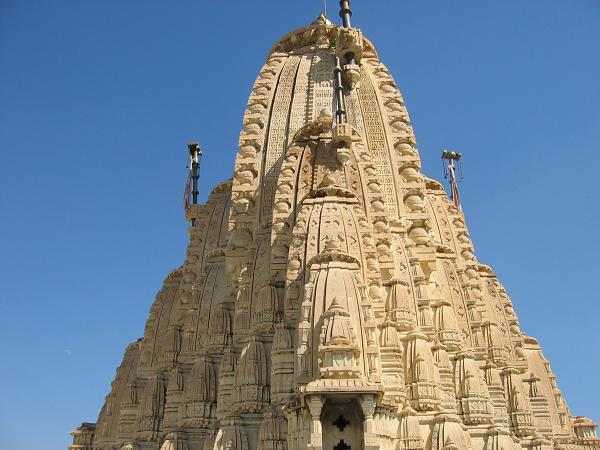
\includegraphics[width=4.8cm]{articles/Octopussy/jain.jpg}
Un temple Jain

Puis nous avons visite le City Palace, d'où la vue sur la ville est superbe.

\hspace*{-0.65cm}
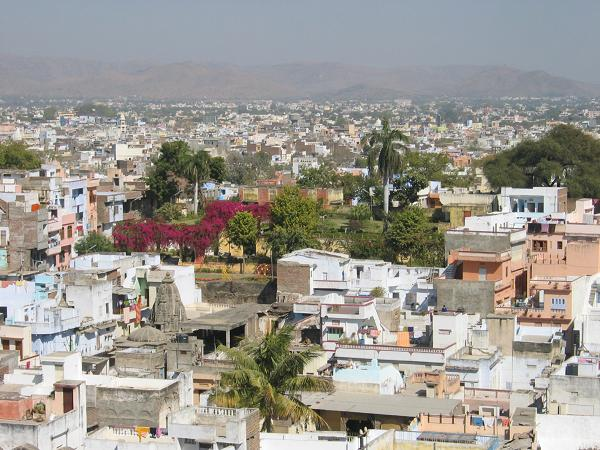
\includegraphics[width=4.8cm]{articles/Octopussy/zoomville.jpg}
Vue sur la ville

Udaipur est aussi connu pour avoir servi de décor au tournage du film Octopussy, James Bond. C'est un luxueux hôtel en plein milieu du lac qui est filmé.

\hspace*{-0.65cm}
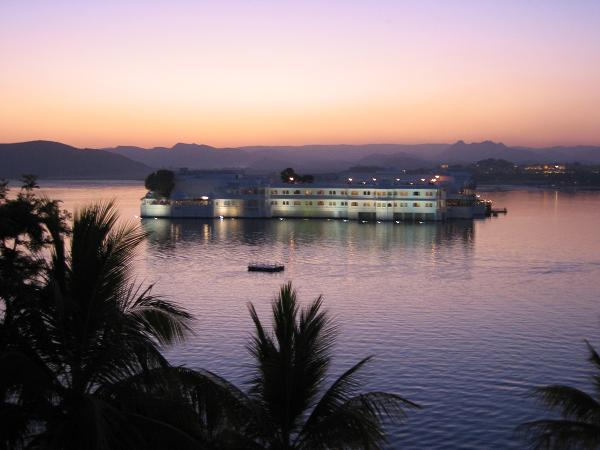
\includegraphics[width=4.8cm]{articles/Octopussy/octopussy.jpg}
Hotel de James Bond

Et pour finir cet article, voici un magnifique coucher de soleil sur le lac.

\hspace*{-0.65cm}
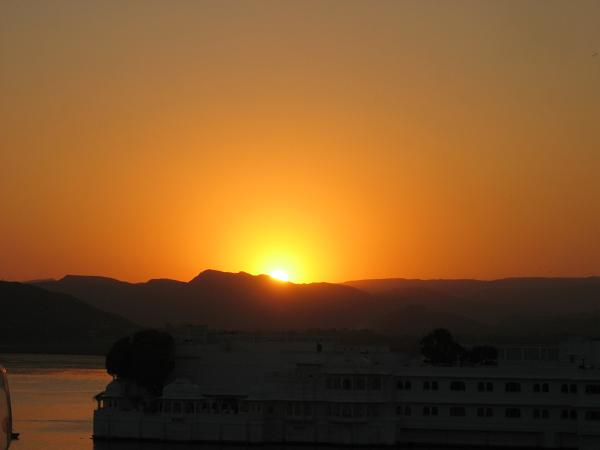
\includegraphics[width=4.8cm]{articles/Octopussy/soleil.jpg}
Coucher de soleil

A bientôt...

\end{multicols}
